% Prepared by Calvin Kent
%
% Assignment Template v19.02
%
%%% 20xx0x/MATHxxx/Crowdmark/Ax
%
\documentclass[12pt]{article} %
\usepackage{CKpreamble}
\usepackage{CKassignment}
\usepackage{tkz-euclide}
\usepackage{physics}
\usepackage{lmodern}
\usepackage{microtype}
\usepackage{tasks}
\usepackage{upgreek}
\usepackage{xcolor}
\usepackage{euscript}
\usepackage{tasks}
\usepackage{upgreek}
\usepackage[misc]{ifsym}


\usepackage{pgfplots}
\usepgfplotslibrary{polar}
\usepgflibrary{shapes.geometric}
\usetikzlibrary{calc}


\usepackage{euscript}
\usepackage{microtype}
\usepackage{upgreek}
\usepackage[misc]{ifsym}

%%Title
\title{Functions Final Exam}
\date{February 3, 2021}

%%% Maths and science packages

\usepackage{amsmath,amsthm,amssymb}
\usepackage{pgfplots}
	\usetikzlibrary{
		calc,
		patterns,
		positioning
	}
	\pgfplotsset{
		compat=1.16,
		samples=200,
		clip=false,
		my axis style/.style={
			axis x line=middle,
			axis y line=middle,
			legend pos=outer north east,
			axis line style={
				->,
			},
			legend style={
				font=\footnotesize
			},
			label style={
				font=\footnotesize
			},
			tick label style={
				font=\footnotesize
			},
			xlabel style={
				at={
					(ticklabel* cs:1)
				},
				anchor=west,
				font=\footnotesize,
			},
			ylabel style={
				at={
					(ticklabel* cs:1)
				},
				anchor=west,
				font=\footnotesize,
			},
			xlabel= $x$,
			ylabel=$\vec d (\m \tx{[East]})$
		},
	}
	\tikzset{
		>=stealth
	}

\pgfplotsset{my style/.append style={axis x line=middle, axis y line=
middle, xlabel={}, ylabel={}, axis equal }}


%%% Tables and figures packages

\usepackage{float}
\usepackage{caption}
	\captionsetup{
		format=plain,
		labelfont=bf,
		font=small,
		justification=centering
	}
	
%%% Numbers and sets

\newcommand{\E}{\mathrm{e}}

\newcommand{\tx}[1]{\text{#1}}

\begin{document}
    \pagenumbering{arabic}
    % Start of class settings ...
    \renewcommand*{\coursecode}{MCR3U Quiz} % Quiz Title
    \renewcommand*{\assgnnumber}{1} % Quiz number
    \renewcommand*{\submdate}{November, 2021} % renew the date
    \renewcommand*{\studentfname}{\textbf{Name:}} % Student first name
    \renewcommand*{\studentlname}{} % Student last name
    %\renewcommand*{\studentnum}{SNumber} % Student number

    \renewcommand\qedsymbol{$\blacksquare$}
    \setfigpath
    % End of class settings 
    \newgeometry{left=18mm, right=18mm, top=22mm, bottom=22mm} % page is set to default values
    \fancyhfoffset[L,O]{0pt} % header orientation fixed
    % End of class settings
    %%% Note to user:
    % CTRL + F <CHANGE ME:> (without the angular brackets) in CKpreamble to specify graphics paths accordingly.
    % The command \circled[]{} accepts one optional and one mandatory argument.
    % Optional argument is for the size of the circle and mandatory argument is for its contents.
    % \circled{A} produces circled A, with size drawn for letter A. \circled[TT]{A} produces circled A with size drawn for TT.
    % https://github.com/CalvinKent/My-LaTeX
    %%%
    % Crowdmark assignment start


    %%%%%%%%%%%%%%%%%%%%%%%%%%%%%%%%%%%%%%%%%%%%%%%%%%%%%%%%%%%%%%%%%%%%%%%%%%%%%%%%%%%%%%%%%%%%%%%%%%%%%%%%
    %%%%%%%%%%%%%%%%%                  PROBLEM IDEAS                  %%%%%%%%%%%%%%%%%%%%%%%%%%%%%%%%%%%%%%
    %%%%%                   ----------------------------------------                                %%%%%%%%

    % --> Do a hard tangent line problem

	\maketitle
	\section{Preamble}
	This final exam covers everything we have learned in this course, with emphasize towards material after test 2. 
  Student's \emph{\textbf{must show all work}} to receive full marks.
	\section{Allowed Aids}
	The following aids are allowed on the Test
	\begin{itemize}
		\item Pencil, Pen, Eraser, Highlighter, Ruler, Protractor, Spare sheets of \textbf{blank} paper.
		\item Reference sheet \textbf{(Double sided paper preprepared by student)}
	\end{itemize}
	\section{Restrictions:}
  \begin{itemize}
		\item \textbf{NO} calculator's.
  \end{itemize}
  \section{Remarks:}
  \begin{itemize}
    \item $\sqrt{xy} = \sqrt{x} \sqrt{y}$.
    \item $\sqrt{x} \sqrt{y} = \sqrt{xy}$.
  \end{itemize}
	\section{Name and Date:}

  \vspace*{0.1cm}

	\begin{center}
	\noindent\begin{tabular}{ll}
		\makebox[3in]{\hrulefill} & \makebox[3in]{\hrulefill}\\
		Name & Date\\[8ex]% adds space between the two sets of signatures
	\end{tabular}
	\end{center}
	\newpage


\section*{Part A - Multiple Choice}
\begin{qstn} % qnumber, qname, qpoints
  Answer the following True/False questions,
  \begin{enumerate}
    \item Let $\mathcal{S} = \{1,2,3\}$, then $\mathcal{S} + \mathcal{S} = \mathcal{S} + \mathcal{S} +
      \mathcal{S}$.\\ 
      Circle the correct answer: \,\, \textbf{True} \,\,\,\,\,\, \textbf{False}

    \item $\left(\sqrt{4} + \sqrt{64} \right) \not \in \mathbb N$.\\
      Circle the correct answer: \,\, \textbf{True} \,\,\,\,\,\, \textbf{False}

    \item The number $29$ is a prime number.\\
      Circle the correct answer: \,\, \textbf{True} \,\,\,\,\,\, \textbf{False}

    \item Let $T = \{x \in \Z \mid \left|x\right| = -1\} $, then $T$ is \textbf{not} empty.\\
      Circle the correct answer: \,\, \textbf{True} \,\,\,\,\,\, \textbf{False}

    \item The vertex of 
      \[
        g(x) = 3\left( x + \sqrt{4}  \right)^2 - 4^2  
      \] is $(-4,-4)$.\\ 
      Circle the correct answer: \,\, \textbf{True} \,\,\,\,\,\, \textbf{False}

    \item The vertex of,
      \[
            H(x) = -\left( x + 2 \right)^2 + 1
      .\] represents a minimum.\\
      Circle the correct answer: \,\, \textbf{True} \,\,\,\,\,\, \textbf{False}

    \item Let $f(x) = \sqrt{x}$. Suppose we apply the following transformations to $f$,
      \begin{itemize}
        \item Reflection across the x-axis.
        \item Vertical stretch by a factor of $2$. 
        \item Horizontal compression by a factor of $2$.
        \item Horizontal shift, right by $2$ units.
        \item Vertical shift, down by $4$ units.
      \end{itemize}
      Then the corresponding transformation equation is $h(x) = -2f(2x - 4) - 4$.\\
      Circle the correct answer: \,\, \textbf{True} \,\,\,\,\,\, \textbf{False}

    \item Let $f(x) = \left|x\right|$, and let $h(x) = -f(2x + 4) - 5$ be a transformation of $f(x)$, then the
      corresponding coordinate transformation of $f$ is,
       \[
           \left( x,f(x) \right)  \longrightarrow \left( \frac{x + 4}{2}, -f(x) - 5 \right) 
      .\] 
      Circle the correct answer: \,\, \textbf{True} \,\,\,\,\,\, \textbf{False}

    \item Let $f \colon \R \to \R$, $f(x) = 2\sqrt{x} + 1$ be a function. Then $f$ is not invertible. \\
      \textbf{Hint: }Try using the Horizontal line test.\\
      Circle the correct answer: \,\, \textbf{True} \,\,\,\,\,\, \textbf{False}

      \newpage

    \item Let $ \mathcal{X} = \{45^{\circ}, 60^{\circ}, 240^{\circ}\} $ and 
      $ \mathcal{Y} = \left\{0,1,\sqrt{3} \right\} $ be sets, define the
            following function, 
            \begin{itemize}
              \item $\mathcal{\omega} \colon \mathcal{X} \to \mathcal{Y}$.
              \item $\mathcal{\omega}(x) = \tan(x)$.
            \end{itemize}
            Then $\omega$ is an invertible function.\\
          Circle the correct answer: \,\, \textbf{True} \,\,\,\,\,\, \textbf{False}

    \item Let $\triangle PQR$ be a \textbf{right triangle} with angle $\angle PQR = 60^{\circ}$ and 
        \textit{hypotenuse} $PQ = 8$. Then $QR = 4$.\\
          Circle the correct answer: \,\, \textbf{True} \,\,\,\,\,\, \textbf{False}

    \item The exact value of 
      \[ 
        \sin 150^{\circ} \cdot \sec 240^{\circ} + \tan 240^{\circ}\tan 30^{\circ} = 0
      \]
      Circle the correct answer: \,\, \textbf{True} \,\,\,\,\,\, \textbf{False}

    \item Let $\triangle PQR$ be a \textbf{right triangle} with $PQ = 6$ and $QR = 3\sqrt{3}$. Then, $\angle PQR = 60^{\circ}$.
      \begin{center}
          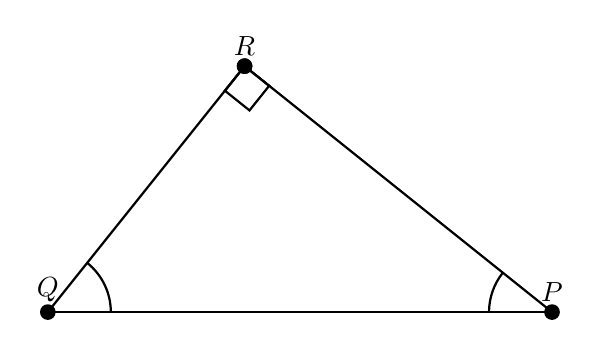
\begin{tikzpicture}[thick]
          \coordinate (Q) at (0,2);
          \coordinate (R) at (2.49878019,5.123475);
          \coordinate (P) at (6.403124,2);

          \draw[black] (0,2) -- (6.403124,2) node[circle,fill,inner sep=2pt]{} node[above]{$P$};
          \draw[black] (0,2) -- (2.49878019,5.123475) node[circle,black,fill,inner sep=2pt]{} node[above]{$R$};
          \draw[black] (6.403124,2) -- (2.49878019,5.123475) node[circle,black,fill,inner sep=2pt]{};
          \draw[black] (0,2) node[circle,black,fill,inner sep=2pt]{} node[above]{$Q$};

          \tkzMarkRightAngle[size=0.4,opacity=1](Q,R,P)% square angle here

          \tkzMarkAngle[fill= orange,size=0.8cm,%
          opacity=1](P,Q,R)
          \tkzLabelAngle[pos = 1.2](P,Q,R){}

          \tkzMarkAngle[fill= orange,size=0.8cm,%
          opacity=1](R,P,Q)
          \tkzLabelAngle[pos = 1.2](R,P,Q){}


          \end{tikzpicture}
      \end{center}
      Circle the correct answer: \,\, \textbf{True} \,\,\,\,\,\, \textbf{False}

    \item $\sin 330^{\circ} = -0.5$.\\
      Circle the correct answer: \,\, \textbf{True} \,\,\,\,\,\, \textbf{False}

    \item Suppose we have the standard coordinates $\vb P\left( 2 , -\sqrt{12}\right) $, then the corresponding polar coordinates
        are $\vb P(4,60^{\circ})$.\\
      Circle the correct answer: \,\, \textbf{True} \,\,\,\,\,\, \textbf{False}

    \item $\sqrt{4^{4}\cdot 3^{2}\cdot 2} = 48\sqrt{2}$. \\
      Circle the correct answer: \,\, \textbf{True} \,\,\,\,\,\, \textbf{False}

  \end{enumerate}
\end{qstn}

\newpage

\section*{Part B}
\begin{qstn}
  Explain in your own words, what is a function?
\end{qstn}

\vspace*{3.5cm}

\begin{qstn}
  Given a function $f \colon A \to B$, explain in your own words, what is the definition of the range of $f$, 
  $\mathcal{R}_f$, what does it contain? Is it necessarily true that $\mathcal{R}_f = B$?
\end{qstn}

\vspace*{5cm}

\begin{qstn}
  Given a function $f \colon A \to B$, explain in your own words, what do we mean when we say that $f$ is
  invertible?
\end{qstn}

\vspace*{5cm}

\begin{qstn}
  Explain what the horizontal line test is as well as the vertical line test.
\end{qstn}

\newpage

\section*{Part C}

\begin{qstn}
  Let $F(x) = x^3  + 1$, and $G(x) = 2x^2 + x - 1$ be functions,
  \begin{enumerate}[label=(\alph*)]
    \item Compute $F(-1)$.
      \vspace*{4cm}

    \item Compute  $G(2)$. 
      \vspace*{4cm}

    \item Compute $F(G(1))$. 
      \vspace*{5cm}

    \item Compute $G(F(F(0)))$.
  \end{enumerate}
\end{qstn}

\newpage

\begin{qstn}
  Let $g(x) = 2x^2 - 4x + 4$,
  \begin{enumerate}[label=(\alph*)]
    \item How many solutions will $g(x)$ have?
      \vspace*{5cm}

    \item Convert $g(x)$ into vertex form by completing the square.
      \vspace*{12cm}

    \item Does the vertex of $g(x)$ represent a minimum or maximum, justify your answer.

  \end{enumerate}
\end{qstn}

\newpage

\begin{qstn}
  Determine the inverse function for the following functions,
  \begin{enumerate}[label=(\alph*)]
    \item $F(x) = -8x + 16$.
        \vspace*{8cm}

    \item $G(x) = 2\sqrt{x + 8} - 4$.
  \end{enumerate}
\end{qstn}

\newpage
\begin{qstn}
Simplify the following exponential expression, \textbf{leave your answer with positive exponents}.
\[
   \frac{\left(2x^2x^4y^{-3}z^{-4} \right)^{2}}{\left(8x^{-2}y^{-5}z^{2} \right)^{2}}
\] 

\end{qstn}

\vspace*{9cm}


\begin{qstn}
  Evaluate the following,
\[
      \left( 16^{\frac{4}{4}} \right) \left( 9^{\frac{3}{2}} \right) \left( 4^{\frac{1}{2}} \right) \left( 2^{-3}
      \right)
\] 
\end{qstn}

\newpage
\begin{qstn}
  Simply the following radical expressions.
  \begin{enumerate}[label=(\alph*)]
    \item \[
        2\sqrt{27} + 3\sqrt{3} - 2\sqrt{12} + \sqrt{48}  
    \] 

    \vspace*{5cm}

  \item \[
      \left( 2\sqrt{2} + \sqrt{3} \right) \left( 5\sqrt{3}  + 3\sqrt{2}\right)
  \] 
  \end{enumerate}
\end{qstn}

\newpage

\begin{qstn}
  Simplify the following,
  \begin{enumerate}[label=(\alph*)]
    \item \[
        \frac{2x^2 - 8x}{x^2 - 11x + 18} \times \frac{2x^{2} - 7x + 6}{x^2 - 5x + 4}
    \] 

    \newpage

  \item \[
      \frac{x}{x^2 - 5x + 6} - \frac{3}{x^2 - 4x + 4}
  \] 
  \end{enumerate}

\end{qstn}

\newpage

\begin{qstn}
 For each of the following, you are given a trigonometric ratio, solve for $\theta$. 
  Assume that each angle  $\theta$ lies in the \textbf{fourth} quadrant.
  \textbf{(You can use the circle below if it helps)}.
  \begin{enumerate}[label=(\alph*)]
    \item \[
      \cos \theta_1 = \frac{1}{2}
    .\] 
   \begin{center}
    \begin{tikzpicture}
      \begin{axis}[
          my style,
          ytick=\empty,
          xtick=\empty,
          xticklabels=\empty,
          width=0.7\textwidth,
          height=0.55\textwidth,
          yticklabels=\empty,
        ]

        \draw (axis cs: 0, 0) circle [radius=20];% I've set the radius to 10 only for better show the image

        \addplot[domain=-21:21, white]{-x};

      \end{axis}
    \end{tikzpicture}
   \end{center}

   \newpage

    \item \[
      \tan \theta_2 = -\frac{1}{\sqrt{3}} 
    .\] 
   \begin{center}
    \begin{tikzpicture}
      \begin{axis}[
          my style,
          ytick=\empty,
          xtick=\empty,
          xticklabels=\empty,
          width=0.7\textwidth,
          height=0.55\textwidth,
          yticklabels=\empty,
        ]

        \draw (axis cs: 0, 0) circle [radius=20];% I've set the radius to 10 only for better show the image

        \addplot[domain=-21:21, white]{-x};

      \end{axis}
    \end{tikzpicture}
   \end{center}

  \end{enumerate}
\end{qstn}

\newpage

\section*{Part D - Solve one of the two problems}

\begin{qstn}
  Suppose we have two standard coordinates $\vb P(x_1,y_1)$ and $\vb Q(x_2,y_2)$. Recall that the distance between
  these two points is given by the following formula,
  \[
        \operatorname{dist} = \sqrt{\left( x_2 - x_1 \right) ^2 + \left( y_2 - y_1 \right) ^2} 
  .\] 

  Given polar coordinates $\vb R(2,150^{\circ})$ and $ \vb T(2,330^{\circ})$, compute the distance between them.
\end{qstn}

\vspace*{1cm}

\begin{qstn}
The figure below is composed of a kite and a circle. The radius of the circle is $4$ and the point $M$
represents the midpoint of the circle. $\angle ADM = 30^{\circ}$ and $MC = 20$. If the area of the circle is $A_c =
48$, then determine the area of the shaded region \emph{in exact form}.\\ (\textbf{Hint:} A kite has unqiue symmetric relationships which assert that
$\angle ADM = \angle ABM$,  $\angle MDC = \angle MBC$, $DM = MB$,  $AD = AB$,  $BC = DC$).
        \begin{center}
          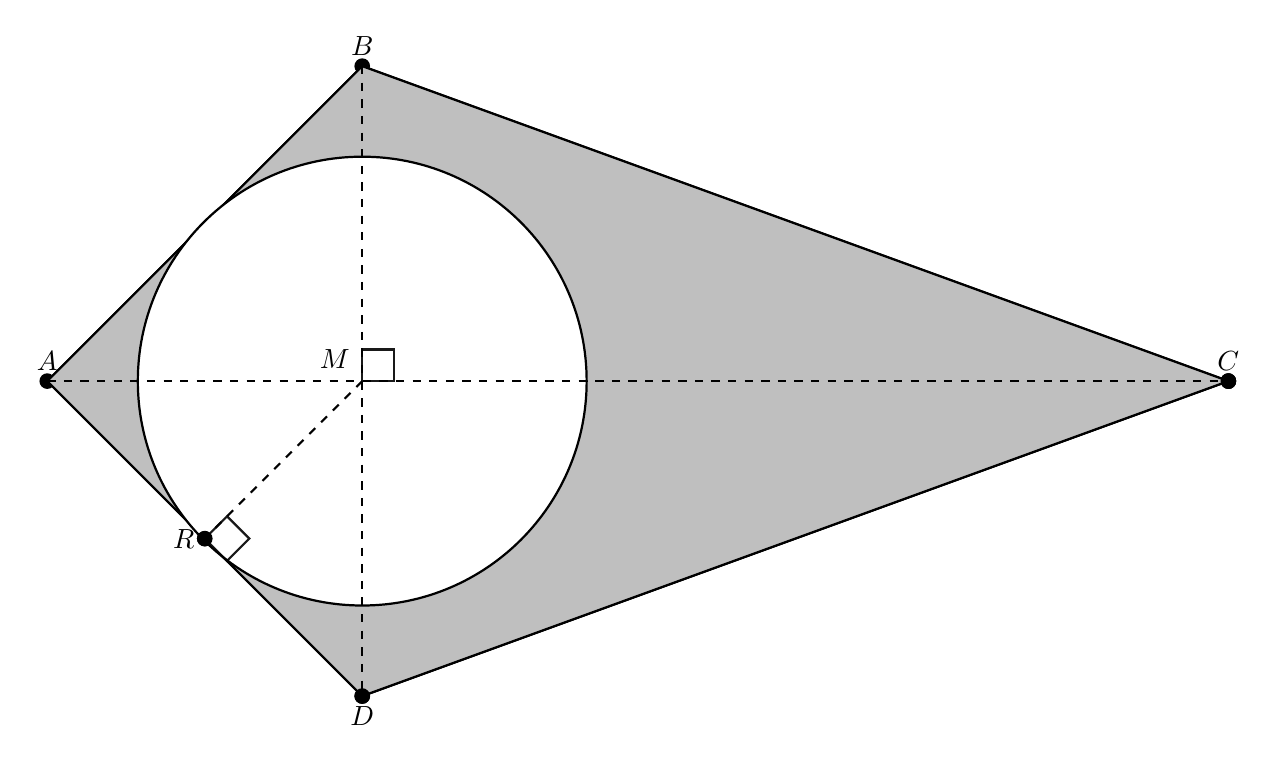
\begin{tikzpicture}[thick]
          \coordinate (A) at (0,0);
          \coordinate (B) at (4,4);
          \coordinate (D) at (4,-4);
          \coordinate (M1) at (2,-2);
          \coordinate (C) at (15,0);
          \coordinate (M) at (4,0);



          \draw[black] (A) -- (B) node[circle,black,fill,inner sep=2pt]{} node[above]{$B$};
          \draw[black] (A) -- (D) node[circle,black,fill,inner sep=2pt]{} node[below]{$D$};
          \draw[black] (B) -- (C) node[circle,black,fill,inner sep=2pt]{} node[above]{$C$};;
          \draw[black] (D) -- (C) node[circle,black,fill,inner sep=2pt]{};
          \draw[black] (A) node[circle,black,fill,inner sep=2pt]{} node[above]{$A$};
          \draw[black] (M1) node[circle,black,fill,inner sep=2pt]{} node[left]{$R$};
          \draw[black] (M) node[circle,black,fill,inner sep=2pt]{};

          \draw[fill=gray!50]  (A) -- (B) -- (C) -- (D) -- cycle;

          \draw[fill=white] (4,0) circle [radius=2.85];% I've set the radius to 10 only for better show the image
          \draw[dashed] (B) -- (D) node[circle,black,fill,inner sep=2pt]{};
          \draw[dashed] (A) -- (C) node[circle,black,fill,inner sep=2pt]{};
          \draw[dashed] (M) -- (M1) node[circle,black,fill,inner sep=2pt]{};

          \tkzMarkRightAngle[size=0.4,opacity=0.9](B,M,C)% square angle here
          \tkzMarkRightAngle[size=0.4,opacity=0.9](M,M1,D)% square angle here

          \node[label={135:{\textcolor{black}{$M$}}},circle,inner sep=0.5pt] at (4,0) {};

          \end{tikzpicture}

      \end{center}
  
\end{qstn}

\vspace*{3cm}

\textbf{\large{CHOOSE AND SOLVE ON NEXT PAGE}}
 
\newpage

\textbf{Question} \underline{\hspace*{1cm}}.\\
\textbf{(You can use the circle below if it helps)}
   \begin{center}
    \begin{tikzpicture}
      \begin{axis}[
          my style,
          ytick=\empty,
          xtick=\empty,
          xticklabels=\empty,
          width=0.8\textwidth,
          height=0.65\textwidth,
          yticklabels=\empty,
        ]

        \draw (axis cs: 0, 0) circle [radius=20];% I've set the radius to 10 only for better show the image

        \addplot[domain=-21:21, white]{-x};


      \end{axis}
    \end{tikzpicture}
   \end{center}

\newpage
\vspace*{2cm}

\end{document}






























